\chapter{Blockchain}
Alla base della più moderna forma di commercio, incentrata sulle criptovalute, troviamo una delle forme di commercio più antica mai messa agli atti. Infatti, il viaggio all'interno della Blockchain e le criptovalute ha inizio nel 1400 d.C. in una piccola isola della Micronesia, l'isola di Yap.

\section{L'isola di Yap}
In una zona remota del Pacifico meridionale si trova un'isola chiamata Yap. Intorno all'isola si trovano migliaia di grandi dischi di calcare e aragonite, disposti in modo casuale. Questi dischi possono essere alti fino a 12 piedi e pesare più di cinquecento chili.

Duemila anni fa, i primi Yapesi (come sono conosciuti) avevano bisogno di creare un sistema di commercio. Poiché sull'isola non c'erano né oro né argento, dovevano trovare un altro materiale che servisse da moneta. Per risolvere questo problema, gli abitanti di Yap trovarono una soluzione creativa. I più forti yapesi navigarono fino all'isola più vicina, a circa 250 miglia di distanza, e riportarono migliaia di grandi massi, di granito che scolpirono in dischi, poi chiamati Rai. A causa delle loro dimensioni, sarebbe stato impossibile spendere questi dischi come il denaro moderno. Invece, i dischi furono collocati in luoghi pubblici in tutta l'isola e non furono mai spostati. All'inizio del sistema di Yap, tutti dovevano ricordare chi possedeva ogni pietra. Man mano che il sistema diventava più complesso, gli abitanti di Yap usavano libri, noti come \textbf{libri mastri}, per registrare chi possedeva ogni pietra. Quando gli yapesi volevano spendere le loro pietre, annunciavano il cambio di proprietà all'intera comunità e tutti aggiornavano i loro libri mastri. In questo modo, gli yapesi potevano spendere le loro pietre senza doverle mai spostare.

Nasce così il libro mastro dalla necessità di monitorare gli scambi senza muovere fisicamente i Rai, nonché il concetto di blockchain, la cui effettiva introduzione e conseguente utilizzo all'nterno di sistemi informatici avviene nella fine del XX secolo.

\begin{figure}[htbp]
  \centering
  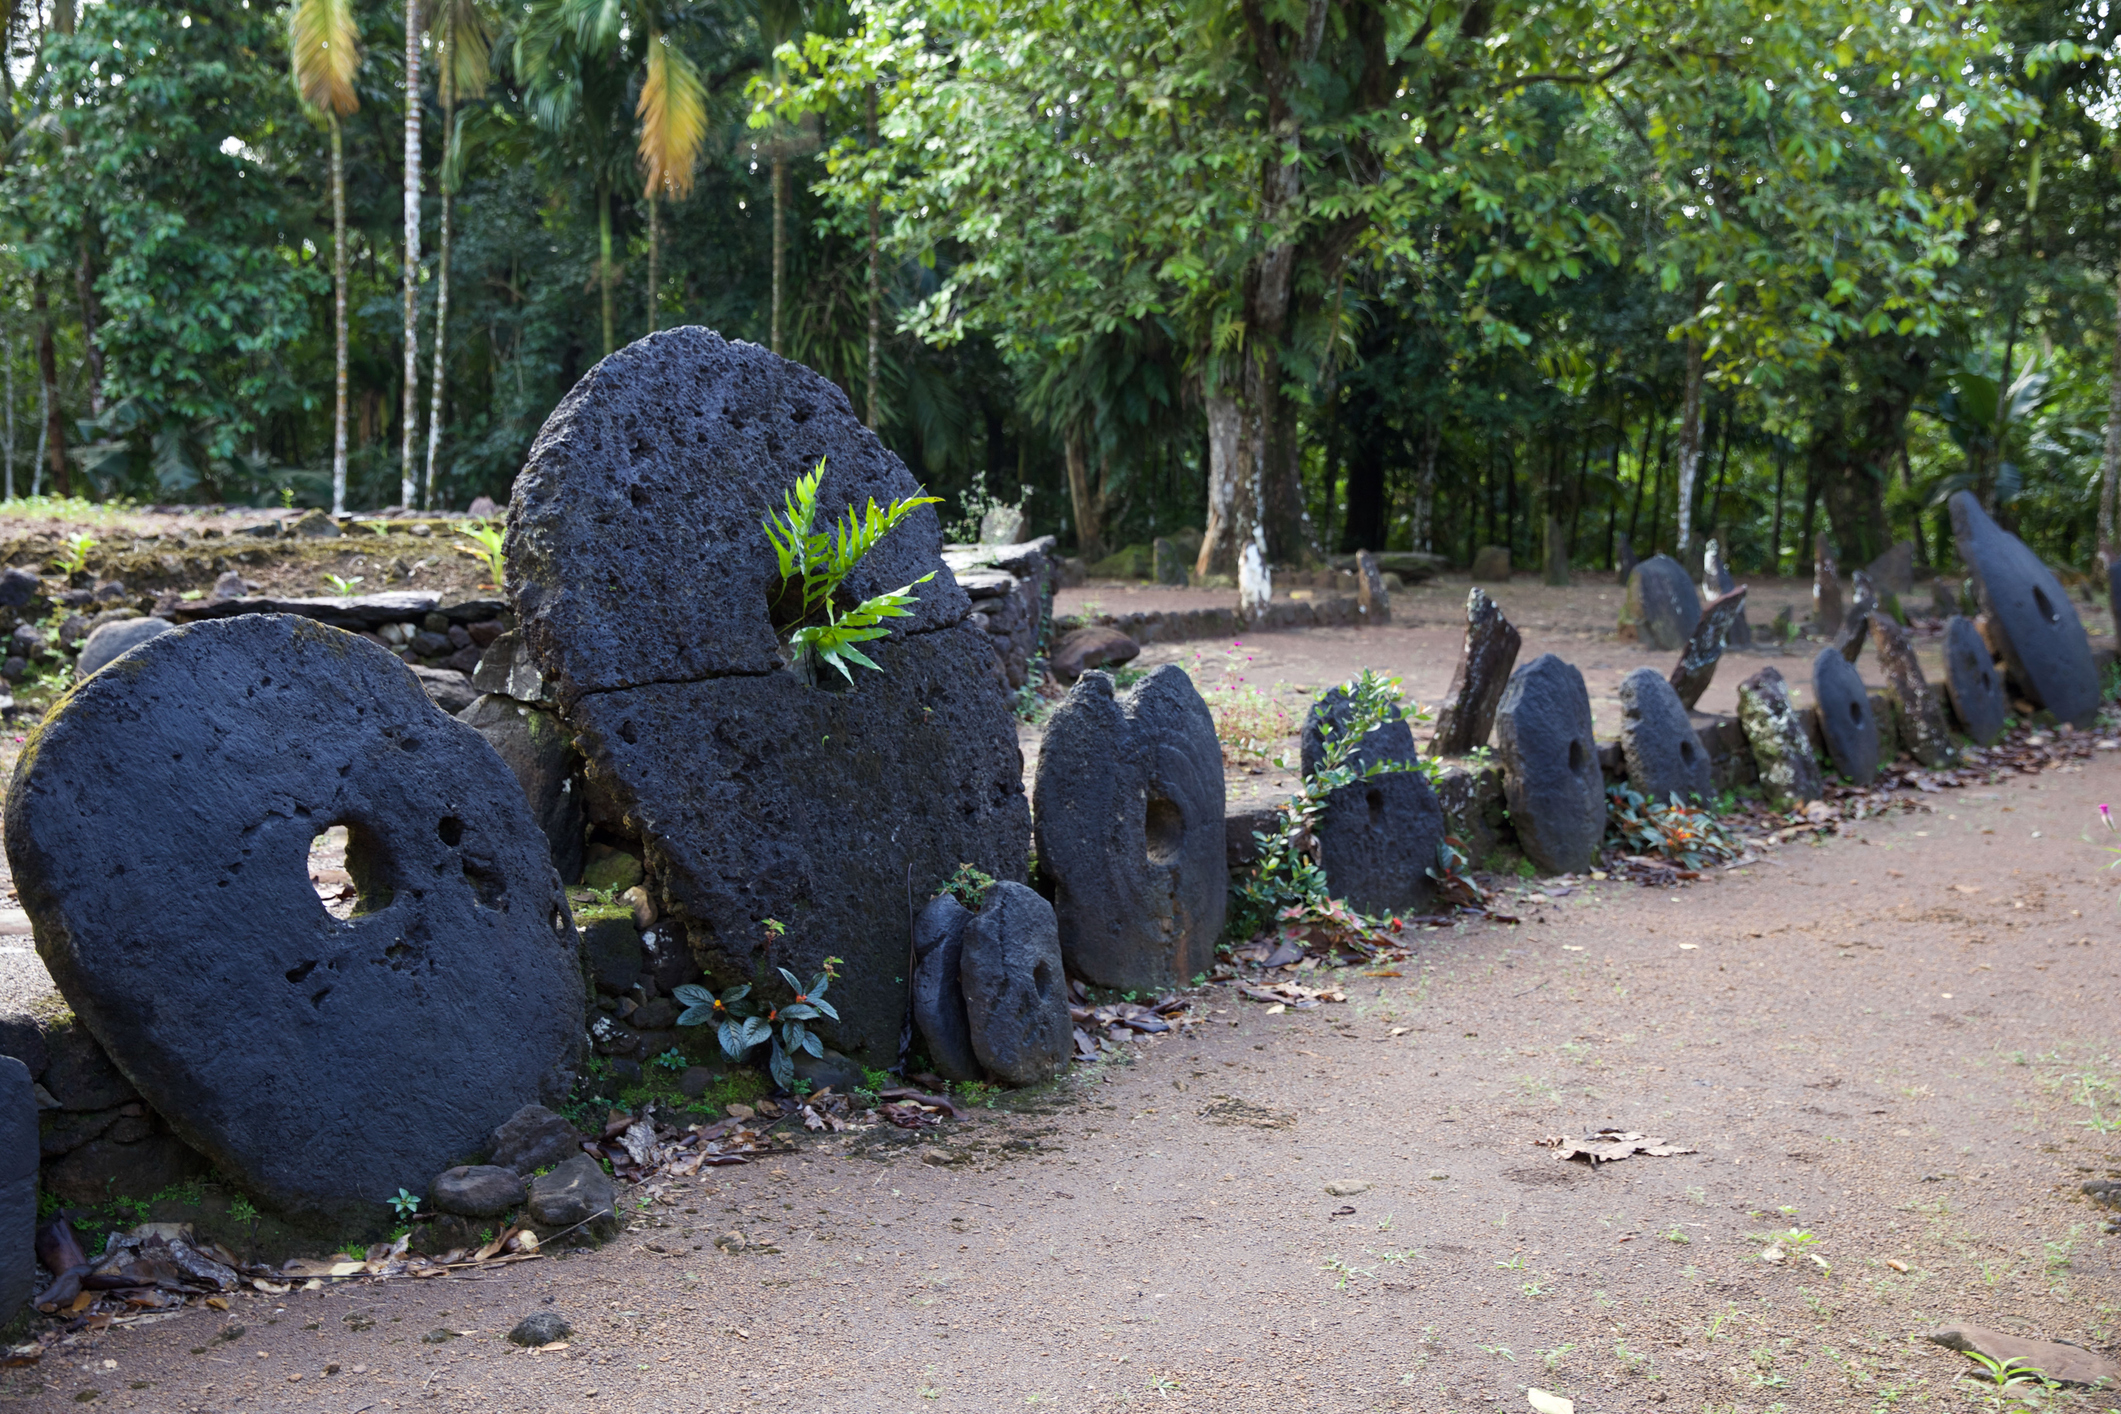
\includegraphics[width=0.8\textwidth]{rai.jpeg}
  \caption{Alcuni Rai dell'isola di Yap}
  \label{fig:rai}
\end{figure}

\section{La storia della Blockchain}

L'evoluzione della blockchain può essere riassunta nei seguenti passaggi principali mostrati nella tabella temporale \ref{tab:blockchain_evolution}.

Nel 1982, il crittografo David Chaum ha proposto per la prima volta un protocollo simile alla blockchain nella sua tesi del 1982 \textit{"Computer e sistemi creati, mantenuti e resi attendibili da gruppi di individui reciprocamente sospettosi"} \cite{computer_systems_chaum}, da qui in poi li definiamo \textbf{Sistemi di Chaum}. Siamo così difronte alla prima idea di tecnologia blockchain.

\begin{table}[htbp]
  \centering
  \scalebox{1.2}{
    \begin{tabular}{r | @{\foo} l}
      1982 & Sistemi di Chaum \newline \\
      1991 & Timestamp \newline \\
      1992 & Alberi di Merkle \newline \\
      2005 & Bitgold \newline \\
      2008 & Bitcoin \\
    \end{tabular}
  }
  \caption{Evoluzione della Blockchain}
  \label{tab:blockchain_evolution}
\end{table}

\subsection{Introduzione ai Sistemi di Chaum}
Probabilmente, molti degli elementi delle blockchain odierne sono contenuti nel sistema di caveau di David Chaum del 1979, descritto nella sua tesi di laurea del 1982 a Berkeley. Chaum descrive la progettazione di un sistema informatico distribuito che può essere creato, mantenuto e reso attendibile da gruppi di individui reciprocamente sospettosi.

Si tratta di un sistema contenente record in grado di manetere la sicurezza e la privacy dei singoli individui tramite sicurezza fisica. Gli elementi costitutivi di questo sistema includono "caveau" fisici (sicuri), primitive crittografiche (crittografia simmetrica e asimmetrica, funzioni hash crittografiche e firme digitali), e una nuova primitia introdotta da Chaum.

\subsection{Timestamp}
Un ulteriore lavoro su una catena di blocchi protetta da crittografia è stato descritto nel 1991 da Stuart Haber e W. Scott Stornetta \cite{haber1990time}. Essi volevano implementare un sistema in cui i timestamp dei documenti non potessero essere manomessi, oggi considerata la prima applicazione della blockchain.

L'utilizzo del timestamp richiede il superamento di due problematiche:

\begin{itemize}
  \item I dati DEVONO essere contrassegnati con l'ora esatta
  \item Il calendario DEVE essere immutabile
\end{itemize}

I due, idearono una soluzione a queste problematiche, definita "naive", la quale consisteva nell'utilizzo di una \textit{cassetta di sicurezza digitale}. Ogni volta che un cliente ha un documento da marcare temporalmente, lo trasmette a un servizio di marcatura temporale (TSS). Il servizio registra la data e l'ora di ricezione del documento e ne conserva una copia. Se l'integrità del documento del cliente viene messa in discussione, viene confrontata con la copia conservata dal TSS. Se le due copie sono identiche, è la prova che il documento non è stato manomesso dopo la data riportata nei registri del TSS.

Questa procedura soddisfa di fatto il requisito centrale per la marcatura temporale di un documento digitale. Tuttavia, questo approccio solleva diverse preoccupazioni:

\begin{description}
  \item[Privacy] Questo metodo compromette la privacy del documento in due modi: una terza parte potrebbe origliare mentre il documento viene trasmesso e, dopo la trasmissione, il documento è a disposizione del TSS stesso. Il cliente deve quindi preoccuparsi non solo della sicurezza dei documenti che tiene sotto il suo diretto controllo, ma anche della sicurezza dei suoi documenti presso il TSS.
  \item[Larghezza di banda e archiviazione] Sia il tempo necessario per inviare un documento per la marcatura temporale che la quantità di memoria richiesta al TSS dipendono dalla lunghezza del documento da marcare. Pertanto, il tempo e la spesa necessari per la marcatura temporale di un documento di grandi dimensioni potrebbero essere proibitivi. 
  \item[Incompetenza] La copia del documento inviata al TSS potrebbe essere danneggiata durante la trasmissione al TSS, potrebbe essere marcata in modo errato quando arriva al TSS, oppure potrebbe essere danneggiata o persa del tutto in qualsiasi momento mentre è conservata presso il TSS. Ognuno di questi eventi invaliderebbe la richiesta di marcatura temporale del cliente.
  \item[Fiducia] Il problema fondamentale rimane: nulla in questo schema impedisce al TSS di accordarsi con un cliente per affermare di aver apposto la data e l'ora su un documento diverso da quello reale.
\end{description}

\subsection{Alberi di Merkle}

\subsection{Bitgold}

\subsection{Bitcoin}
\[\begin{tikzcd}
	{H_0 = Hash (Client \; A \; crea \; il \; documento) \; istante \; di \; tempo \; i} & {} \\
	{H_1 = Hash (Client \; B \; aggiunge \; una \; pagina) \; istante \; di \; tempo \; i+1} \\
	{H_2 = Hash (Client \; C \; corregge \; gli \; errori \; di \; spelling) \; istante \; di \; tempo \; i+2}
	\arrow[from=1-1, to=2-1]
	\arrow[shift right=5, curve={height=30pt}, from=2-1, to=1-1]
	\arrow[from=2-1, to=3-1]
	\arrow[shift right=5, curve={height=30pt}, from=3-1, to=2-1]
\end{tikzcd}\]
